\documentclass[12pt,a4paper]{article}

\usepackage[letterpaper]{geometry}

\usepackage{times}
\geometry{top=1.0in, bottom=1.5in, left=1.0in, right=1.0in}

\usepackage{fancyhdr}
\pagestyle{fancy}
\lhead{}
\rhead{}
\lfoot{}
\rfoot{}

\renewcommand{\headrulewidth}{0pt} 
\renewcommand{\footrulewidth}{0pt} 

\setlength\headsep{0.333in}

\usepackage{fontspec}
%\setmainfont{Times New Roman}

\usepackage{graphicx}

\usepackage{hyperref}

\usepackage{caption}

\usepackage{indentfirst}

\usepackage{setspace}

\usepackage{float}

\usepackage{enumitem}
\usepackage{listings}
\usepackage{color}
\usepackage{xcolor}

\usepackage{tabularx}

\usepackage{amsmath}

\begin{document}

\begin{titlepage}

\newcommand{\HRule}{\rule{\linewidth}{0.5mm}}

\center

\textsc{\LARGE UM - SJTU Joint Institute}\\[1cm]
\textsc{\Large Physics Laboratory I}\\[0.5cm]
\textsc{\large VP141}\\[0.5cm]

\HRule \\[0.4cm]
{
    \bfseries
    {\huge Exercise II}\\[0.3cm]
    {\large Measurement of Fluid Viscosity}\\[0.2cm]
    \HRule \\[1.5cm]
}

\begin{minipage}{0.6\textwidth}

\large
\emph{Name:}\\
Tianyi \textsc{Ge} \\

\emph{Student Number:}\\
516370910168 \\

\emph{Group:}\\
17\\

\emph{Instructor:}\\
Prof. Mateusz \textsc{Krzyzosiak}

\end{minipage}\\[3.5cm]

{\large \today}\\[2cm]

\vfill

\end{titlepage}

%\setmainfont{Times New Roman}
\onehalfspacing 
\newpage

\section{Introduction}

The objective of this exercise is to study damped and driven oscillations in
mechanical systems using the Pohl resonator. For driven oscillations, we will
also observe and quantify the mechanical resonance phenomenon. 
    
If a periodically varying external force is applied to a damped harmonic
oscillator, the resulting motion is called forced (or driven) oscillations, and
the external force is called the driving force. Assuming that the driving force
is of the form 
    \[
        F=F_0(sin\omega t+\delta),
    \]
with the amplitude F 0 and angular frequency ω, the resulting steady-state
forced oscillations will be simple harmonic with the angular frequency equal to
that of the driving force. The amplitude of these steady-state oscillations
turns out to depend on the angular frequency of the the driving force, in
particular on how far it is from the natural angular frequency, and the damping
coefficient. The amplitude may become quite large, and this phenomenon is known
as the mechanical resonance. 

Another interesting property of driven steady-state oscillations is the fact
that there is a phase lag between the driving force and the displacement from
the equilibrium position of the oscillating particle. This phase lag reaches
$\pi/2$ (a quarter of the cycle) when the system is driven at the natural
angular frequency.
    
In this experiment, forced oscillation of a balance wheel will be studied. The
corresponding quantities (such as the force and the position) will be replaced
by their angular counterparts. 

The driving torque $\tau_{dr}=\tau_0cos\omega t$ and a damping torque
$\tau_f=-b\frac{d\theta}{dt}$, Also, we know the restoring torque
$\tau=-k\theta$, its equation od motion is of the form 

\begin{equation}
\label{1}
I\frac{d^2\theta}{dt^2}=-k\theta-b\frac{d\theta}{dt}+\tau_0cos\omega t,
\end{equation}

where I is the moment of inertia of the balance wheel, $\tau_0$ is the amplitude
of the driving torque, and $\omega$ is the angular frequency of the driving
torque. Introducing the symbols 

\[
\omega_0=\frac{k}{I},\quad 2\beta=\frac{b}{I}, \quad \mu=\frac{\tau_0}{I}, 
\]

Eq. \ref{1} can be rewitten as
\begin{equation}
\label{2}
\frac{d^2\theta}{dt^2}+2\beta\frac{d\theta}{dt}+\omega_0^2\theta
=\mu cos\omega t.
\end{equation}

Thw solution to Eq \ref{2} is
\[
\theta(t)=\theta_{tr}(t)+\theta_{st}cos(\omega t+\varphi),
\]
where the former term $\theta_{tr}$ denotes the transient solution that vanished
exponentially as $t\rightarrow \infty$. The steady-state  oscillation is with
the amplitude 
\[
\theta_{st}=\frac{\mu}{\sqrt{(\omega_0^2-\omega^2)^2+4\beta^2\omega^2}}
\]
For small values of the damping coefficient \beta, the resonance angular
frequency is close to the the natural angular frequency, and the amplitude of
steady-state oscillations becomes large. The dependence of both the amplitude
and the phase shift on the driving angular frequency are shown in the left and
right Figure 1, respectively, for different values of the damping coefficient.

\newpage
%\section{Measurement Method}


%\section{Measurement Procedue}


%\section{Caution}
\begin{itemize}
\item Do not move the graduated flask during the measurement.
\item Be careful with the castor oil: do not spill it on the desk.  
\item Do not forget to read the ambient temperature, as fluid viscosity is
  sensitive to the temperature. 
\end{itemize}



%\section{Result}

\section{Results}

\subsection{Measurement for natural angular frequency}
We calculate the angular frequency from Table~\ref{data_omega} by the formula
\[
\omega_0=\frac{2\pi}{T}.
\]
\begin{table}[H] 
\centering
\begin{tabular}{|c|c|}
\hline
& $10T[s] \pm 0.001[s]$\\\hline
1 & 15.790  \\\hline
2 & 15.801  \\\hline
3 & 15.778  \\\hline
4 & 15.800  \\\hline
\end{tabular}
\caption{Measurement of ten periods for the natural frequency}
\label{data_omega}
\end{table}

Hence the average value of $10T$ should be calculated as

\[
\overline{10T}=\frac{1}{4}\sum_{i=1}^{4}(10T)_i=15.79225 \pm 0.0107 \ s, \quad
u_{10T,r}=0.07\%. 
\]

The value of $\omega_0$ is

\[
\overline{\omega_0}=\frac{20\pi}{10T}=\frac{20\times3.1416}{15.79225}= 3.9787
\pm 0.006 \  rad/s,\quad u_{\omega_0,r}=0.15\%. 
\]

\subsection{Measurement for damping coefficient}

The damping coefficient can be calculated by the following formula.

\[
\beta=\frac{1}{5T}\ln\frac{\theta_i}{\theta_{i+5}}.
\]


In the experiment, we choose Damping Selection 2.

\begin{table}[H] 
\centering

\begin{tabular}{|c|c|c|c|c|}
\hline

\multicolumn{2}{|c}{Amplitude[$\degree$]$\pm$1[$\degree$]} & 
\multicolumn{2}{|c|}{Amplitude[$\degree$]$\pm$1[$\degree$]} &
$\ln(\theta_i/\theta_{i+5})$\\\hline

$\theta_0$ & 149 & $\theta_5$ & 95 & 0.4501 \\\hline
$\theta_1$ & 136 & $\theta_6$ & 86 & 0.4583 \\\hline
$\theta_2$ & 124 & $\theta_7$ & 79 & 0.4508 \\\hline
$\theta_3$ & 114 & $\theta_8$ & 72 & 0.4595 \\\hline
$\theta_4$ & 103 & $\theta_9$ & 65 & 0.4603 \\\hline
\multicolumn{4}{|c|}{The average value of $\ln(\theta_i/\theta_{i+5})$}
    & 0.4558 \\\hline 
\end{tabular}

\caption{Measurement of the damping coefficient for Damping Selection 2}
\label{data_damping}
\end{table}

The experimental value of $\ln(\theta_i/\theta_{i+5})$ is shown below

\[
\ln(\theta_i/\theta_{i+5})= 0.4558 \pm 0.0050 , \quad u_r=1.09\%
\]

Here, $T= 15.79225 /10= 1.5792 \pm 0.0001s$. Then we can easily obtain $\beta$
as well, 

\[
\beta=\frac{1}{5\times1.5792}\times0.4558=  0.0577 \pm 0.003s^{-1}, \quad
u_{\beta,r}=5.2\% 
\]

\subsection{Measurement for $\theta_{st}$ vs. $\omega$ and $\varphi$ vs. 
  $\omega$} 

To study the relation between $\varphi$ and $\omega/\omega_0$, 

first we get the raw data of 10T, $\phi$ and $\theta$,
we then process the raw data and list them in Table~\ref{data_phi2} and
Table~\ref{data_phi3}. 


\begin{table}[H]
\centering
\begin{tabular}{|c|c|c|c|}
\hline
& $10T [s] \pm 0.001 [s]$ &  $\varphi  [\degree]  \pm 1 [\degree]$ & $ \theta [\degree] \pm 1 [\degree]$ \\ \hline

1  & 15.098 & -162  &  38   \\ \hline
2  & 15.123 & -163  &  39   \\ \hline
3  & 15.542 & -143  &  87   \\ \hline
4  & 15.672 & -118  &  130  \\ \hline
5  & 15.707 & -109  &  138  \\ \hline
6  & 15.724 & -103  &  141  \\ \hline
7  & 15.736 & -100  &  143  \\ \hline
8  & 15.755 & -94   &  145  \\ \hline
9  & 15.763 & -92   &  146  \\ \hline
10 & 15.774 & -89   &  144  \\ \hline
11 & 15.788 & -86   &  144  \\ \hline
12 & 15.797 & -84   &  144  \\ \hline
13 & 15.810 & -82   &  144  \\ \hline
14 & 15.820 & -79   &  142  \\ \hline
15 & 15.841 & -75   &  140  \\ \hline
16 & 15.907 & -64   &  130  \\ \hline
17 & 15.946 & -57   &  124  \\ \hline
18 & 16.050 & -46   &  105  \\ \hline
19 & 16.131 & -40   &  92   \\ \hline
20 & 16.237 & -33   &  78   \\ \hline
21 & 16.472 & -22   &  54   \\ \hline
22 & 16.603 & -18   &  46   \\ \hline
\end{tabular}    
\caption{$\theta$ vs. $10T$ and $\varphi$ vs. $10T$ raw data for Damping selection 2}
\end{table}

\begin{table}[H]
\centering
\begin{tabular}{|c|c|c|c|}
\hline
& $10T [s] \pm 0.001 [s]$ &  $\varphi  [\degree]  \pm 1 [\degree]$ & $ \theta [\degree] \pm 1 [\degree]$ \\ \hline

1  & 15.057   & -163 &  35   \\ \hline
2  & 15.302   & -155 &  50   \\ \hline
3  & 15.526   & -142 &  79   \\ \hline
4  & 15.657   & -123 &  108  \\ \hline
5  & 15.708   & -111 &  120  \\ \hline
6  & 15.745   & -104 &  125  \\ \hline
7  & 15.760   & -97  &  127  \\ \hline
8  & 15.794   & -93  &  128  \\ \hline
9  & 15.789   & -92  &  128  \\ \hline
10 & 15.803   & -89  &  128  \\ \hline
11 & 15.814   & -86  &  128  \\ \hline
12 & 15.830   & -83  &  128  \\ \hline
13 & 15.849   & -80  &  126  \\ \hline
14 & 15.883   & -74  &  124  \\ \hline
15 & 15.903   & -69  &  120  \\ \hline
16 & 15.933   & -62  &  114  \\ \hline
17 & 16.013   & -55  &  106  \\ \hline
18 & 16.102   & -47  &  93   \\ \hline
19 & 16.168   & -41  &  83   \\ \hline
20 & 16.290   & -33  &  70   \\ \hline
21 & 16.452   & -25  &  55   \\ \hline
22 & 16.585   & -18  &  46   \\ \hline
\end{tabular}    
\caption{$\theta$ vs. $10T$ and $\varphi$ vs. $10T$ raw data for Damping selection 3}
\end{table}


Then We know that $ \omega / \omega_0 = T_0 / T $,
thus we can have the following processed data.


\begin{table}[H]
\centering
\begin{tabular}{|c|c|c|}
\hline
& $\omega/\omega_0$ &  $\varphi \pm 1 [\degree] $ \\ \hline
1  & 1.0460  & -162  \\ \hline
2  & 1.0443  & -163  \\ \hline
3  & 1.0161  & -143  \\ \hline
4  & 1.0077  & -118  \\ \hline
5  & 1.0054  & -109  \\ \hline
6  & 1.0043  & -103  \\ \hline
7  & 1.0036  & -100  \\ \hline
8  & 1.0024  & -94   \\ \hline
9  & 1.0019  & -92   \\ \hline
10 & 1.0012  & -89   \\ \hline
11 & 1.0003  & -86   \\ \hline
12 & 0.9997  & -84   \\ \hline
13 & 0.9989  & -82   \\ \hline
14 & 0.9982  & -79   \\ \hline
15 & 0.9969  & -75   \\ \hline
16 & 0.9928  & -64   \\ \hline
17 & 0.9904  & -57   \\ \hline
18 & 0.9839  & -46   \\ \hline
19 & 0.9790  & -40   \\ \hline
20 & 0.9726  & -33   \\ \hline
21 & 0.9587  & -22   \\ \hline
22 & 0.9512  & -18   \\ \hline
\end{tabular}    
\caption{$\varphi$ vs. $\omega/\omega_0$, Damping selection 2}\label{data_phi2}
\end{table}

\begin{table}[H]
\centering
\begin{tabular}{|c|c|c|}
\hline
& $\omega/\omega_0$ &  $\varphi \pm 1 [\degree] $ \\ \hline
1  & 1.0488   & -163 \\ \hline
2  & 1.0320   & -155 \\ \hline
3  & 1.0171   & -142 \\ \hline
4  & 1.0086   & -123 \\ \hline
5  & 1.0054   & -111 \\ \hline
6  & 1.0030   & -104 \\ \hline
7  & 1.0020   &  -97 \\ \hline
8  & 0.9999   &  -93 \\ \hline
9  & 1.0002   &  -92 \\ \hline
10 & 0.9993   &  -89 \\ \hline
11 & 0.9986   &  -86 \\ \hline
12 & 0.9976   &  -83 \\ \hline
13 & 0.9964   &  -80 \\ \hline
14 & 0.9943   &  -74 \\ \hline
15 & 0.9930   &  -69 \\ \hline
16 & 0.9912   &  -62 \\ \hline
17 & 0.9862   &  -55 \\ \hline
18 & 0.9808   &  -47 \\ \hline
19 & 0.9768   &  -41 \\ \hline
20 & 0.9694   &  -33 \\ \hline
21 & 0.9599   &  -25 \\ \hline
22 & 0.9522   &  -18 \\ \hline
\end{tabular}    
\caption{$\varphi$ vs. $\omega/\omega_0$, Damping selection 3}\label{data_phi3}
\end{table}




\begin{figure}[H]
\centering
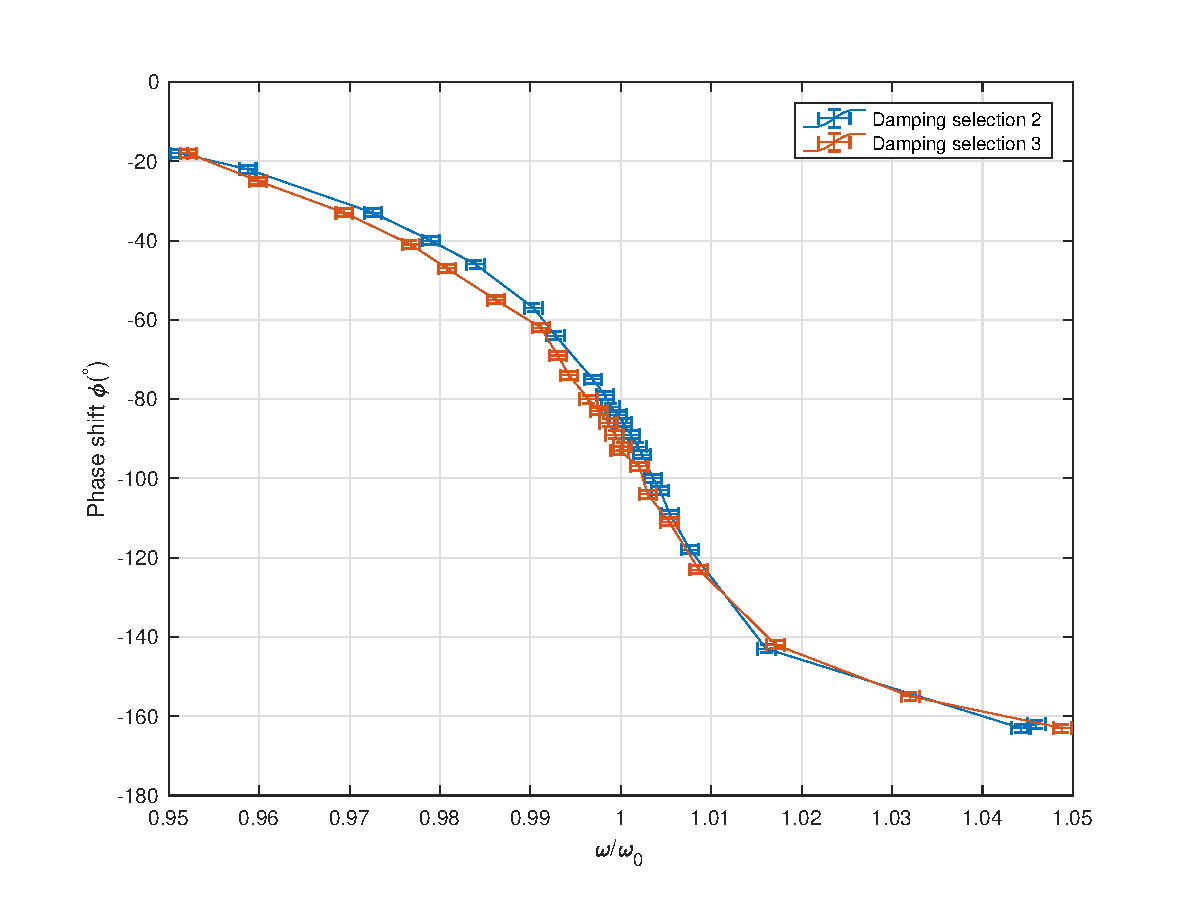
\includegraphics[width=1\textwidth]{matlab/p1}
\caption{Phase shift $\varphi$ vs. $\omega/\omega_0$}\label{phi}
\end{figure}


To study the relation between $\theta_{st}$ and $\omega/\omega_0$, we process the raw data and list them in Table~\ref{data_t2} and Table~\ref{data_t3}.


% TODO:







\begin{table}[H]
\centering
\begin{tabular}{|c|c|c|}
\hline
& $\omega/\omega_0$ &  $\theta \pm 1 [\degree] $ \\ \hline
1  & 1.0460  & 38   \\ \hline
2  & 1.0443  & 39   \\ \hline
3  & 1.0161  & 87   \\ \hline
4  & 1.0077  & 130  \\ \hline
5  & 1.0054  & 138  \\ \hline
6  & 1.0043  & 141  \\ \hline
7  & 1.0036  & 143  \\ \hline
8  & 1.0024  & 145  \\ \hline
9  & 1.0019  & 146  \\ \hline
10 & 1.0012  & 144  \\ \hline
11 & 1.0003  & 144  \\ \hline
12 & 0.9997  & 144  \\ \hline
13 & 0.9989  & 144  \\ \hline
14 & 0.9982  & 142  \\ \hline
15 & 0.9969  & 140  \\ \hline
16 & 0.9928  & 130  \\ \hline
17 & 0.9904  & 124  \\ \hline
18 & 0.9839  & 105  \\ \hline
19 & 0.9790  & 92   \\ \hline
20 & 0.9726  & 78   \\ \hline
21 & 0.9587  & 54   \\ \hline
22 & 0.9512  & 46   \\ \hline
\end{tabular}    
\caption{$\theta$ vs. $\omega/\omega_0$, Damping selection 2}\label{data_t2}
\end{table}

\begin{table}[H]
\centering
\begin{tabular}{|c|c|c|}
\hline
& $\omega/\omega_0$ &  $\theta \pm 1 [\degree] $ \\ \hline
1  & 1.0488   & 35   \\ \hline
2  & 1.0320   & 50   \\ \hline
3  & 1.0171   & 79   \\ \hline
4  & 1.0086   & 108  \\ \hline
5  & 1.0054   & 120  \\ \hline
6  & 1.0030   & 125  \\ \hline
7  & 1.0020   & 127  \\ \hline
8  & 0.9999   & 128  \\ \hline
9  & 1.0002   & 128  \\ \hline
10 & 0.9993   & 128  \\ \hline
11 & 0.9986   & 128  \\ \hline
12 & 0.9976   & 128  \\ \hline
13 & 0.9964   & 126  \\ \hline
14 & 0.9943   & 124  \\ \hline
15 & 0.9930   & 120  \\ \hline
16 & 0.9912   & 114  \\ \hline
17 & 0.9862   & 106  \\ \hline
18 & 0.9808   & 93   \\ \hline
19 & 0.9768   & 83   \\ \hline
20 & 0.9694   & 70   \\ \hline
21 & 0.9599   & 55   \\ \hline
22 & 0.9522   & 46   \\ \hline
\end{tabular}    
\caption{$\theta$ vs. $\omega/\omega_0$, Damping selection 3}\label{data_t3}
\end{table}

\begin{figure}[H]
\centering
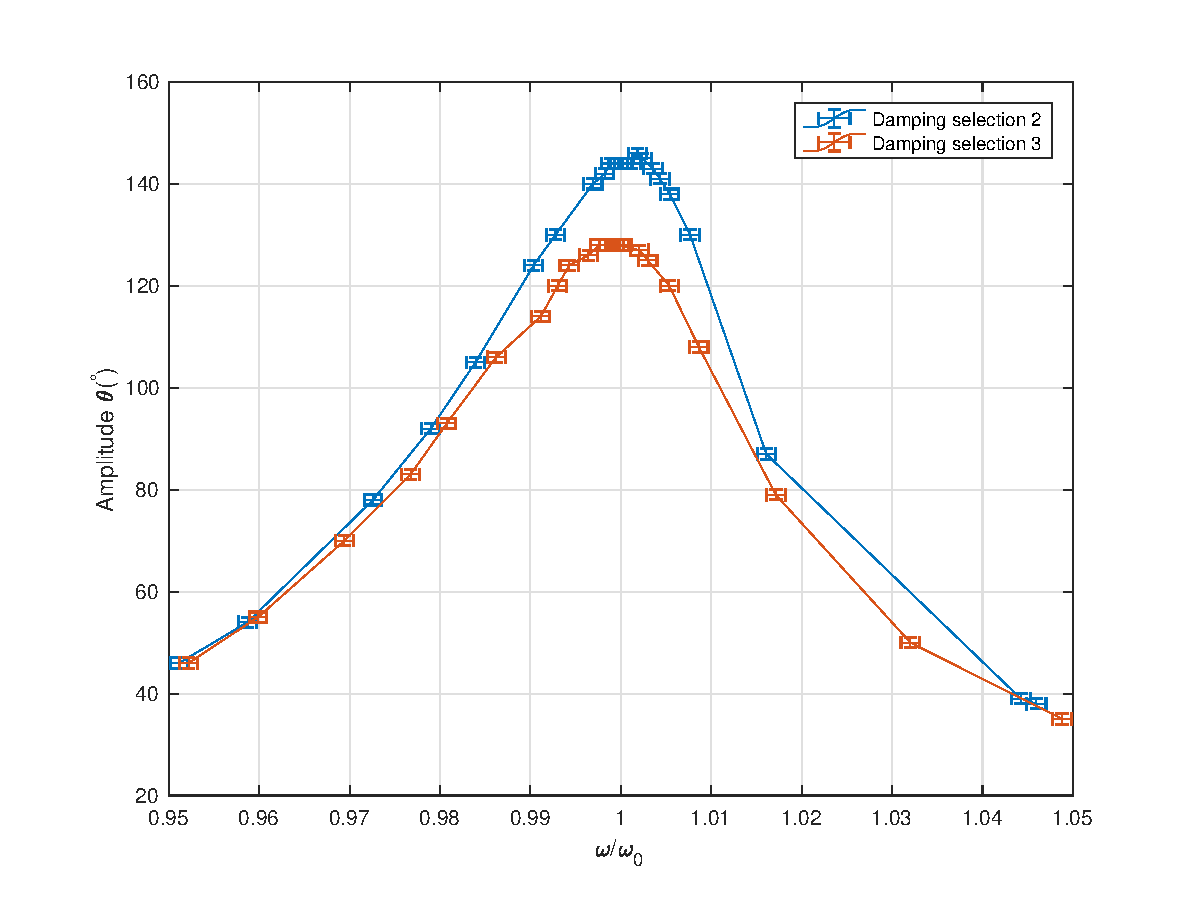
\includegraphics[width=1\textwidth]{matlab/p2}
\caption{Amplitude $\theta_{st}$ vs. $\omega/\omega_0$}\label{theta}
\end{figure}

%\section{Measurement Uncertainty Analysis}

\subsection{Uncertainty of The Distance Measurement}
We use formula to calculate type-A uncertainty
\begin{multline*}
 u_A = t_{0.95} \sqrt{\frac{1}{3(3-1)} \sum_{k=1}^3{(S_k-\bar{S})^2} } = \\
4.30 \cdot \sqrt{1/6\cdot ( (147.0-  146.83)^2 +  (147.0-  146.83)^2 + (146.5-
  146.83)^2 ) } =   0.7 mm
\end{multline*}
And type-B uncertainty is $u_B = $ = 1 mm. Thus,

$$   u_s = \sqrt{u_A^2+u_B^2} = \sqrt{0.7^2+1^2} = 1.2 mm  $$
$$   u_{S,r} = 1.2 / 146.8 = 0.82 \% $$ 

\subsection{Uncertainty of The Time Measurement}
We use formula to calculate type-A uncertainty
\begin{equation}
 u_A = t_{0.95} \sqrt{\frac{1}{6(6-1)} \sum_{k=1}^6{(t_k-\bar{t})^2} } = 1.05
 \cdot 0.0252 = 0.0492 s
\end{equation}
And type-B uncertainty is $u_B = $ = 0.01 s. Thus,
$$   u_t = \sqrt{u_A^2+u_B^2} = \sqrt{0.0492^2+0.01^2} =  0.0502 s $$
$$   u_{t,r} = 0.050 / 6.8517= 0.73 \% $$ 


\subsection{Uncertainty of The Ball Diameter}
We use formula to calculate type-A uncertainty
\begin{equation}
  u_A = t_{0.95} \sqrt{\frac{1}{10(10-1)} \sum_{k=1}^{10}{(d_k-\bar{d})^2} }
 = 0.715  \cdot   0.0197 = 0.0141 s
\end{equation}
And type-B uncertainty is $u_B = $ = 0.005 mm. Thus,
$$   u_d = \sqrt{u_A^2+u_B^2} = \sqrt{0.0141^2+0.005^2} = 0.0150 mm $$
$$   u_{d,r} = 0.0150 / 1.977 =  0.76 \% $$ 

\subsection{Uncertainty of The Inner Diameter of The Flask}
We use formula to calculate type-A uncertainty
\begin{equation}
  u_A = t_{0.95} \sqrt{\frac{1}{6(6-1)} \sum_{k=1}^{6}{(D_k-\bar{D})^2} }
 = 1.05  \cdot 0.0523 =  0.0549 mm 
\end{equation}
And type-B uncertainty is $u_B = $ = 0.02 mm. Thus,
$$   u_D = \sqrt{u_A^2+u_B^2} = \sqrt{0.0549^2+0.02^2} = 0.0584 mm $$
$$   u_{D,r} = 0.0584 /  61.3533 =  0.095 \% $$ 

\subsection{Uncertainty of The Inner Diameter of The Flask}
We use formula to calculate type-A uncertainty
\begin{equation}
  u_A = t_{0.95} \sqrt{\frac{1}{6(6-1)} \sum_{k=1}^{6}{(D_k-\bar{D})^2} }
 = 1.05  \cdot 0.0523 =  0.0549 mm 
\end{equation}
And type-B uncertainty is $u_B = $ = 0.02 mm. Thus,
$$   u_D = \sqrt{u_A^2+u_B^2} = \sqrt{0.0549^2+0.02^2} = 0.0584 mm $$
$$   u_{D,r} = 0.0584 /  61.3533 =  0.095 \% $$ 




%\section{Conclusion and Discussion}

For the resonance method and the comparison method
    
In the experiment 
the speed of sound in the air was measured through two ways: 
the resonance method and the phase comparison method. 
From the two means, we have 
    \begin{equation}
    \begin{split}
        v&=351.05\pm0.4 m/s,\quad u_{r,v}=0.10\%;\\
        v&=348.95\pm10 m/s,\quad u_{r,v}=3\%,
    \end{split}
    \end{equation}
    respectively. 

    From the result after analyzing, we can conclude that the results of the resonance method has higher precision but not enough accuracy.
    On the other hand, the results of the phase comparison method has higher accuracy but not enough precision.

The reason account for the lack of  preciseness may be the easiness to 
determine the time we get the distance which shares the same length of half wave length for Resonance Method, 
or one wave length for Phase comparison Method.

For Resonance Method, it's not very easy to observe whether the wave on oscilloscope became the maximum amplitude. 
For Phase-comparison Method, it is easy to observe whether the Lissajous figure becomes a straight line with a positive slope in each period. 

Thus we managed to get the data that are close to each other because of the easy observation. 
The very uncertainty may due to random error in this experiment.

The reason for the preciseness may be that we manage to obverse the place of first resonance point, though the resonance curve is not flat enough, which may make the observation difficult.
 The little relative error may come from random error in this experiment and the difficulty to obverse.

In conclusion, the result produced in the experiment is relatively precise and accurate. 
Through the Resonance Method and the Phase-comparison Method, we can get a very precise result. 
Through the Time-difference Method, we can get a very accurate result, though it may only be an accident in this experiment. In order to compare these four methods, we should do the experiment for several times to reduce random error.
Moreover, we are introduced the Successive Difference Method, which is a more effective way to reduce error. We can use this method in other experiments.


%\section{Reference}
\begin{enumerate}
\item  The international system of units (SI) (PDF) (2008 ed.). United States Department of Commerce, NIST Special Publication 330. pp. 29 \& 57.
\item “Exercise 2-Lab Manual” Qin Tian, Feng Yaming, Mateusz Krzyzosiak,Department of Physics, Shanghai Jiaotong University.  
\end{enumerate}

\section{Data Sheet}

% data sheet

\end{document}